\documentclass{article}
\usepackage[margin=1in]{geometry}
\usepackage{amsmath}
\usepackage{amssymb}
\usepackage{mathtools}
\usepackage{float}
\usepackage{tikz}
\usetikzlibrary{automata, positioning, arrows}
\tikzset{
    ->,
    >=stealth',
    node distance=3cm,
    every state/.style={thick, fill=gray!10}, 
    initial text=$ $, 
}
\title{Title}
\author{Ty Butler}

\newcommand{\thm}[1]{\textbf{Theorem #1}}
\newcommand{\Nat}{\mathbb{N}}
\newcommand{\Int}{\mathbb{Z}}
\newcommand{\Rat}{\mathbb{Q}}
\newcommand{\Real}{\mathbb{R}}
\newcommand{\Comp}{\mathbb{C}}

\begin{document}
\maketitle{}

\section{}
\subsection*{a.}
Suppose there existed no path of width at least $\frac{F}{m}$. Since there are $m$ edges in the graph, there are at most $m$ paths from $s$ to $t$. Since each path has less than $\frac{F}{m}$ capacity, the total capacity of all paths is less than $\frac{F}{m} m = F$. Consider a cut separating $s$ from $t$. Since the maximum capacity of all paths is less than $F$, the capacity of the cut must necessarily be less than $F$, as it encompasses all paths. Since such a cut exists, any minimum cut will also have a capacity less than $F$. Therefore, by the max-flow min-cut theorem, the max flow from $s$ to $t$ is less than $F$. This is a contradiction, as $F$ cannot be less than $F$, and therefore our assumption that no path of width at least $\frac{F}{m}$ exists must be false. 

\subsection*{b.}
The widest path will have a width of at least $\frac{F}{m}$. Therefore, after pushing flow to it, the residual graph will have total capacity $F - \frac{F}{m}$. Therefore the remaining fraction after one round is $1 - \frac{1}{m}$, and so the amount left after $k$ iterations will be $F(1 - \frac{1}{m})^k$. Since $1 - \frac{1}{m}$ is between $0$ and $1$, the amount left must be at most $F(e^-{\frac{1}{m}})^k = F(e^{-\frac{k}{m}})$. We want to find $k$ such that this amount is at most $1$, because at that point we know there is at most $1$ iteration left to bring the residual capacity to zero. This is represented as the inequality $F(e^{-\frac{k}{m}}) \leq 1$, equivalently, $\ln(F(e^{-\frac{k}{m}})) = \ln(F) + \ln(e^{-\frac{k}{m}}) = \ln(F) - \frac{k}{m} \leq 1$. Since we are working asymptotically, "less than 1" is asymptotically equivalent to "equals zero", so we can change the equation back to $\ln(F) - \frac{k}{m} = 0$. This equation further yields $\ln(F) = \frac{k}{m}$, and then $k = m\ln F$, and therefore $k \in O(m \ln F)$. 


\section{}
\subsection*{a.}
Consider the case of three students $s_1, s_2, s_3, s_4$, with groups $(s_1, s_2, s_3), (s_1, s_3, s_4), (s_2, s_3, s_4)$. Since each student is in two groups of size $3$, each student will have total responsibility $\frac{2}{3}$. Since groups must have a note-taker, a student must be chosen to take notes for at least $1$ group, and will thus be assigned to more groups than their responsibility.

\subsection*{b.}
For this problem, we have a set of students $p_1...p_n$, each of whom can be assigned to at most some number $F_1...F_n$ of groups. We have a set of groups $S_1...S_m$, each of which needs exactly one note taker from within its set of students. We want to maximize the number of groups with note takers. We can express these constraints as a bipartite graph. The first set of nodes will be $n$ nodes for the students. For each student $p_j$, there will be an edge from the source node to the student with capacity $F_j$. This represents how the student can serve as note-taker for at most $F_j$ groups. The second set of nodes will be $m$ nodes for the groups. Each group node will be connected to the sink by an edge with capacity $1$. This represents how each group needs one note-taker. For each student $p_j$ and group $S_i$, there will be an edge from $p_j$ to $S_i$ if and only if $p_j$ is in group $S_i$, and this edge will have capacity $1$. The edge will have flow if the student is assigned as a note-taker for the group, and will have no flow otherwise. Thus each student will be connected to the set of groups for which they can be a note-taker. 

Our algorithm will first convert the input problem into the aforementioned graph, then apply the Ford-Fulkerson algorithm to find the maximum flow through the graph. The algorithm will find a valid solution if and only if the maximum flow is equal to $m$. For each group $S_j$, the algorithm will take $q_j$ to be the student to which $S_j$ is connected to by an edge with a flow of $1$. 

\textbf{Claim:} The algorithm will find a valid solution if and only if it finds a valid maximum flow of size $m$.
For each group $S_j$, there is a edge of with $1$ going to the sink. There are $m$ groups, so the capacity directly into the sink consists of $m$ edges of length $1$ coming from the group nodes. 

Suppose there is no valid assignment of note-takers. A valid assignment of note-takers is one such that each group has an assigned note-taker, and no student $p_j$ is assigned to more than $F_j$ groups. Suppose a group has no assigned note-taker. In the graph, this is represented as a group node having no in-edges with flow. Since out flow must equal in flow, the group node must also have no flow on its out edge to the sink node. Since the sink's in-edges consist of $m$ edges of with $1$, if there is an edge with no flow, the total flow into the sink must be less than $m$, and thus the max flow must be less than $m$. 

Suppose the maximum flow is not $m$. Clearly, the maximum flow of the graph is no greater than $m$, as a cut of the graph which removes all of these edges would have a capacity of $m$, so any minimum cut would have a capacity of at most $m$. Therefore we need only to consider the case where the maximum flow is less than $m$. If the maximum flow is less than $m$, the flow into the sink is less than $m$. Since the edges into the sink consist of $m$ edges of width $1$, this means that at least one of these edges has no flow. Consider one of these edges, $e_j$, connected to group $S_j$. Since this edge is the only outlet from $S_j$, $S_j$ must have no in edges with flow, as out flow must equal in flow. Since the in edges to a group $S_j$ represent the students in $S_j$, with flow if the student is assigned as the note-taker, $S_j$ must have no assigned note-taker. Thus if the maximum flow on the graph is not $m$, there does not exist a valid assignment of note-takers.

\textbf{Claim: } If the algorithm has found a max flow of size $m$, the set of student nodes with nonzero flows to group nodes will be a valid solution. 

A valid solution is one in which no group has exactly one assigned note-taker, and each student $p_j$ is assigned as note-taker to no more than $F_j$ groups. Suppose a non-valid solution assigns more than one student to a group. This would be represented within the graph as more than one in-edges to a group $S_j$ having nonzero flow. Since each group has exactly one out-edge with width $1$, this would violate the condition that in-flow equals out-flow, and thus would not be a valid max-flow. Thus, by the contrapositive, if the algorithm finds a max-flow, each group will be assigned at most one note-taker. Suppose a non-valid solution assigns a student $p_j$ to more than $F_j$ groups. This would be represented in the graph by a student node having more than $F_j$ out-edges with nonzero flow. Since each student has exactly one in-edge with width $F_j$, this would violate the condition that in-flow must equal out-flow, and would not be a valid max-flow. Thus, by contrapositive again, if the algorithm finds a max-flow, each student $p_j$ will be assigned to at most $F_j$ groups.

\textbf{Claim:} Building the graph is $O(mn)$.

Given $n$ students and $m$ groups, we assign $m$ edges between the groups and sink ($O(m)$), and then, for each group, we must assign at most $n$ edges, one for each student in the group ($O(mn)$). Then, for each student, we must find their maximum number of groups. Assuming the work to retrieve a group's size is constant, we must retrieve the size of each group for each student, so this step is also $O(mn)$. This results in a total work of $O(m) + O(mn) + O(mn) = O(mn)$. 

\textbf{Claim: } The algorithm is $O(m^2n)$.

The work of the Ford-Fulkerson algorithm for a graph $(V, E)$ with maximum flow $F$ is $O(F(|V| + |E|))$. We established previously that the maximum flow for a valid solution is $m$. The graph for the problem has $m$ group nodes, $n$ student nodes, and a source and sink, so $|V| = 2 + m + n$. The graph has $m$ edges from the group nodes to the sink, and $n$ edges from the source to the student nodes. The graph also has an edge for each student in each group, so with each of $m$ groups having at most $n$ students, there are at most $nm$ edges between the student and group nodes. Therefore $|E| \in O(m + n + mn)$. Therefore the total work of the Ford-Fulkerson algorithm on this graph will be $O(m ((2 + m + n) + (m + n + mn))) = O(m(2 + 2m + 2n + mn)) = O(2m + 2m^2 + 2mn + m^2n) = O(m^2n)$.

In order to find the assigned students after applying the Ford-Fulkerson algorithm, can trace through the resulting flow graph produced by the algorithm. For each group $S_j$, check which in-edge has nonzero flow. The student at the other end of this edge will be $q_j$. As proven previously, there will be only one such student for each group. Since there are $m$ groups and at most $n$ students per group, this process' work is $O(mn)$.

Therefore the overall algorithm has asymptotic complexity $O(mn) + O(m^2n) + O(mn)$, which simplifies to $O(m^2n)$.

\subsection*{c.}

A group of size $n_j$ gives $\frac{1}{n_j}$ responsibility to each of its members. Thus it gives a total of $1$ resposibility to the collective responsibility of all students. This collective responsibility is represented within the graph as the total capacity of all the edges from the source to the students, as for a student $p_j$, the width of the edge $s \rightarrow p_j$ is $F_j$. Thus each group increases the total capacity of the source to student nodes by $1$, so the total capacity of all the source to student edges will be at least $m$ (to account for the possible rounding up). 

Now, consider the Ford-Fulkerson algorithm applied to the graph. Since the edge from any group to the sink has width $1$, and there are $m$ such edges, the total capacity from the groups to the sink will be $m$. We estableshed previously that the total capacity from the source to the students is at least $m$. Additionally, there are as many edges between the groups and students as there are students in groups. In the worst case, each group contains only one student, in which case the total capacity of the edges between the students and the groups is $m$ (as if any group contains more than one student, there will be additional total capacity). 

For each iteration of the algorithm, any valid path will have the same capacity, limited to $1$ by the edges between the groups and the sink. Therefore a single iteration of the algorithm will identify a path which includes one of the source to student edges and one of the group to sink edges, and will push $1$ unit of flow. This reduces the residual capacity of the group to sink nodes by $1$, and also reduces the residual capacity of the source to student nodes by $1$. The algorithm will repeat until there is no path from $s$ to $t$ with nonzero residual capacity. Since the group to sink edges have total capacity $m$ while the source to student and student to group edges each have total capacity of at least $m$, and the total capacity for each is reduced by $1$ each time, this will happen after $m$ iterations. Since there is $1$ flow pushed for each iteration, the maximum flow pushed after $m$ iterations must be $m$. As shown previously, a max flow of $m$ indicates a valid solution exists. $\blacksquare$


\end{document}

\iffalse
example fsm
\begin{figure}
    \centering
    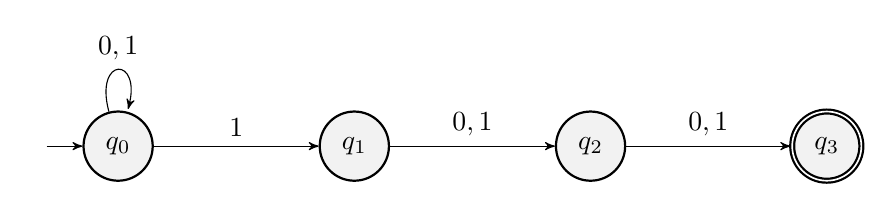
\begin{tikzpicture}
        \node[state, initial] (q0) {$q_0$};
        \node[state, right of=q0] (q1) {$q_1$};
        \node[state, right of=q1] (q2) {$q_2$};
        \node[state, accepting, right of=q2] (q3) {$q_3$};

        \draw 
            (q0) edge[loop above] node{$0,1$} (q0)
            (q0) edge[above] node{$1$} (q1)
            (q1) edge[above] node{$0,1$} (q2)
            (q2) edge[above] node{$0,1$} (q3);
    \end{tikzpicture}
\end{figure}
\fi
